\documentclass{article}

% math, graphics, and formatting
\usepackage{amsmath,amsbsy,amssymb,amsthm,fullpage,graphicx,pgfplots,breqn}
\usepackage{verbatim,mathtools}

% physics
\usepackage{physics}
\newcommand{\h}{\hbar}
\renewcommand{\vec}{\mathbf}

% Times New Roman
\usepackage{newtxtext}
\usepackage{newtxmath}
\renewcommand{\mathbb}{\varmathbb}
%\usepackage{libertine}
%\usepackage[libertine]{newtxmath}

% section numbering: e.g. 2b (ii)
%\renewcommand\thesection{\arabic{section}}
%\renewcommand\thesubsection{\thesection\alph{subsection}}
%\renewcommand\thesubsubsection{\thesubsection\,(\roman{subsubsection})}

% theorems & proofs
\theoremstyle{definition}
\newtheorem*{prop}{Claim}
\newtheorem*{claim}{Claim}
\newtheorem*{prob}{Problem}
\newtheorem*{obs}{Observation}
\newtheorem*{lemma}{Lemma}
\newtheorem*{thm}{Theorem}
\newtheorem*{disc}{Discussion}
\newtheorem*{defn}{Definition}
\newtheorem*{eg}{Example}

% derivatives
\newcommand{\pp}{\partial}
\newcommand{\pd}[2]{\ensuremath\frac{\pp #1}{\pp #2}}
\newcommand{\pdd}[2]{\ensuremath\frac{\pp^2 #1}{\pp #2^2}}
\renewcommand{\dd}[2]{\ensuremath\frac{d#1}{d#2}}
\newcommand{\ddd}[2]{\ensuremath\frac{d^2 #1}{d #2^2}}
\newcommand{\del}{\nabla}

% sets and complex numbers
\newcommand{\R}{\mathbb R}
\renewcommand{\Re}{\textrm{Re}}
\renewcommand{\Im}{\textrm{Im}}
%\renewcommand{\bar}{\overline}
\newcommand{\nin}{\not\in}
\newcommand{\str}[1]{\ensuremath{\langle #1 \rangle}}

% probability and stats
\renewcommand{\var}{\ensuremath\mathbf{Var}}
\newcommand{\E}{\ensuremath\mathbf{E}}
\renewcommand{\P}{\ensuremath\mathbf{P}}

% measurement
\newcommand{\un}[1]{\;\mathrm{#1}}
\newcommand{\ch}[1]{\mathrm{#1}}

% Greek letters are hard
\newcommand{\ep}{\varepsilon}
\newcommand{\om}{\omega}

% formatting
\renewcommand{\sp}[1]{\;\;\;\text{ #1 }\;\;\;}
\newcommand{\cc}{\texttt}
\newcommand{\plop}[2]{
    \begin{figure}\centering
        \includegraphics[width=0.8\textwidth]{#1}
        \caption{\label{#1}#2}
    \end{figure}
}
\newcommand{\sbsplop}[4]{
    \begin{figure}\centering
        \includegraphics[width=0.49\textwidth]{#1}
        \includegraphics[width=0.49\textwidth]{#2}
        \caption{\label{#1}#3}
        {#4}
    \end{figure}
}

\usepackage{fancyhdr}
\usepackage[margin=1in, headheight=50pt]{geometry}
\pagestyle{fancy}
\lhead{\textbf{Ph21 Set 3}}
\chead{}
\rhead{Aritra Biswas}
\setlength{\headsep}{20pt}

\begin{document}

\section{Procedure}

We test our edge detector on the two images shown in Figure
\ref{headphones.jpg}.
The mic and headphones image was obtained from a wallpaper
website\footnote{\texttt{http://www.pickywallpapers.com/1920x1080/music/headphones/studio-mic-with-headphones-wallpaper/download/}}
and the carrots image from a stock image website.\footnote{\texttt{http://pngimg.com/upload/carrot_PNG4985.png}}
\sbsplop{headphones.jpg}{carrots.png}{Headphones and carrots.}{}

We used the Python Imaging Library to import each image and create an
array of RGB tuples. Each component in the tuple was added to get the
brightness of each pixel. We computed the magnitude of the gradient
of this 2D array by using a Gaussian first derivative stencil provided by
\texttt{scipy.ndimage}. This stencil requires a standard deviation $\sigma$
to compute how wide the distribution is, i.e. how many neighbors we take
into account when computing the gradient at a pixel. Results are
shown in figures \ref{headphones_edges} and \ref{carrots_edges}
for $\sigma = 0.5, 1, 3$, and $5$. A smaller choice of $\sigma = 0.2$ yielded
no visible edges for both test images.

\section{Comments}

\subsection{Color limitations}

The magnitude of the gradient shows where the image substantially changes
brightness, indicating an edge. Notably, we only use the brightness
instead of each RGB color component. This works for our images because
real-world edges in photos correlate with large brightness changes. However,
if we were to edge-detect a flag where one band is pure blue $(0, 0, 256)$
and another is pure red $(256, 0, 0)$, the program would fail to find
the edge between these bands.

\subsection{CAPTCHAs}

While edge-detection would be an important step in beating CAPTCHAs,
it is probably not the most difficult step. Some CAPTCHA-like images
simply overlay colored but nicely typed letters on a noisy background.
Edge detection would be the main step in identifying letters in an image
like this. The edges could be passed to OCR.

However, real CAPTCHAs often don't rely on a noisy background. Instead,
they rely on warping the letters, requiring some interpretation of
the edge curvatures and some way to unwarp the image before comparing it
to standard fonts. Edge detection would be required to isolate the
letters from the background, but the unwarping would be the difficult step.

    \begin{figure}\centering
        \frame{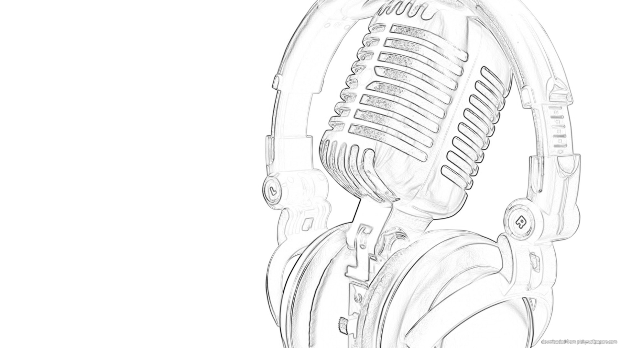
\includegraphics[width=0.49\textwidth]{sig05_headphones.png}}
        \hspace{1mm}
        \frame{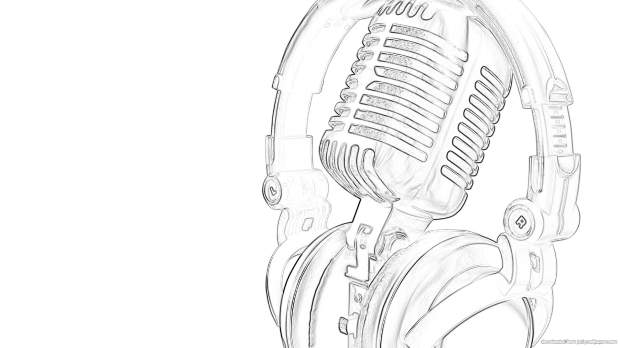
\includegraphics[width=0.49\textwidth]{sig1_headphones.png}}
        \\\vspace{2mm}
        \frame{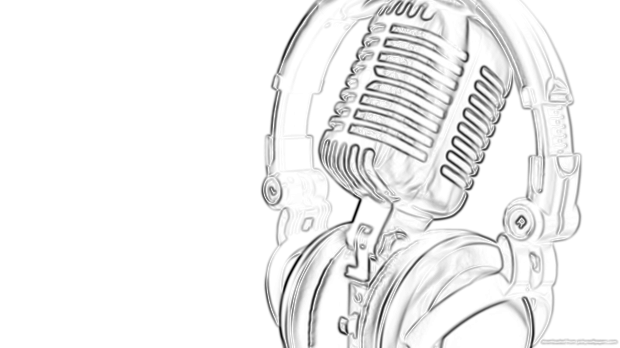
\includegraphics[width=0.49\textwidth]{sig3_headphones.png}}
        \hspace{1mm}
        \frame{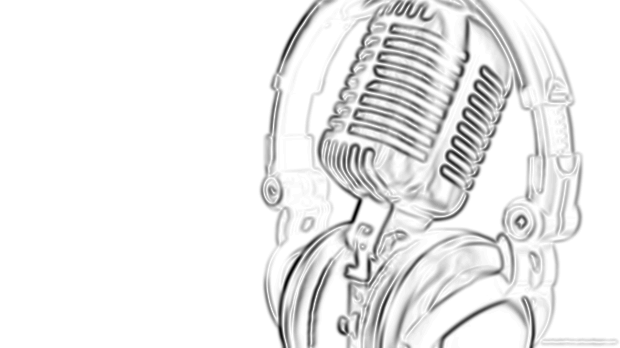
\includegraphics[width=0.49\textwidth]{sig5_headphones.png}}
        \caption{\label{headphones_edges}From top left to bottom right:
        edge detection with $\sigma = 0.5, 1, 3, 5$.}
    \end{figure}
    \begin{figure}\centering
        \frame{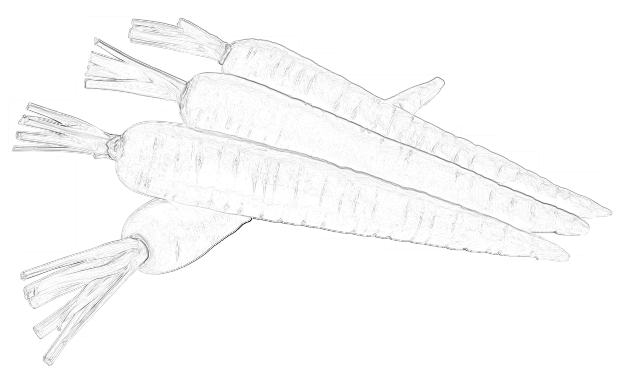
\includegraphics[width=0.49\textwidth]{sig05_carrots.png}}
        \hspace{1mm}
        \frame{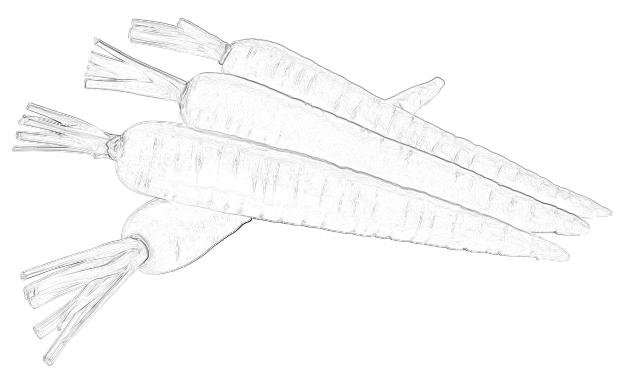
\includegraphics[width=0.49\textwidth]{sig1_carrots.png}}
        \\\vspace{2mm}
        \frame{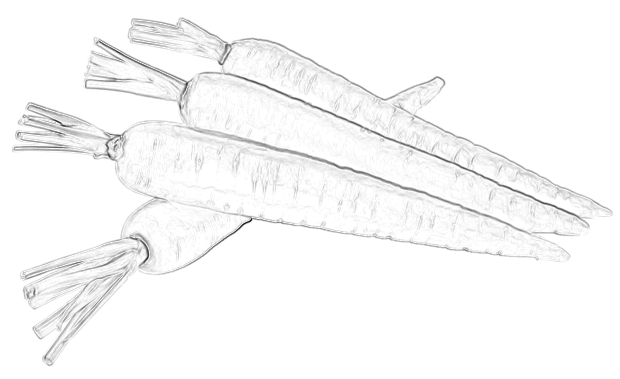
\includegraphics[width=0.49\textwidth]{sig3_carrots.png}}
        \hspace{1mm}
        \frame{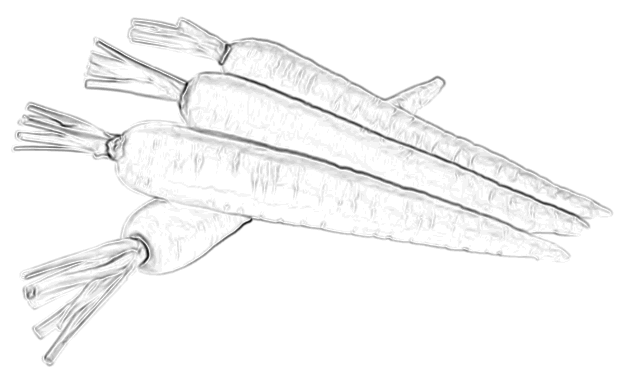
\includegraphics[width=0.49\textwidth]{sig5_carrots.png}}
        \caption{\label{carrots_edges}From top left to bottom right:
        edge detection with $\sigma = 0.5, 1, 3, 5$.}
    \end{figure}

\end{document}
